\subsection{Sprint 3}
\subsubsection{Sprint start}
This sprint was dedicated to work on the customers wishes for the application. A customer meeting had been done on the last day of last sprint. The meeting gave us a lot of good feedback about what to focus on.
What the team experienced had experienced previously was that it was hard to work on writing the application for the parts that was not well prototyped.
The decision thus, was to focus on having detailed, well thought prototypes, that would satisfy the customers feedback. 

For the parts of the application that we don't have time to implement, there will be a textual description.


\subsubsection{Execution of the sprint}
\subsubsection{Development}
\subsubsection{Testing}
\subsubsection{Design}
\subsubsection{Project Administration}

\subsubsection{Sprint burndown}

The sprint burndown chart~\ref{fig:sprint3burndown} shows that some progress was made.

\begin{figure}[H]
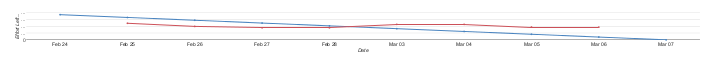
\includegraphics[width=\textwidth]{ch/projectManagement/fig/sprint3burndown.png}
\caption{Sprint 3 burndown chart}
\label{fig:sprint3burndown}
\end{figure}

\subsubsection{Sprint backlog}

The backlog and time usage result.

\begin{tabular}{|l|p{4cm}|c|c|r}%
    \hline \bfseries User story & \bfseries Details & \bfseries Hours estimated & \bfseries Hours spent & \bfseries Hours left
    \csvreader[head to column names]{ch/projectManagement/sec/sprint3/userstories.csv}{}% use head of csv as column names
    {\\\hline \id & \title & \estimated & \spent & \left}% specify your coloumns here
\end{tabular}


\subsubsection{Sprint end}

What

Project status


